\documentclass[xcolor=svgnames]{beamer} %svgnames import a bunch of colors
%to make black and white paste ", blackandwhite" inside brackets above (for transparencies)
\usetheme{Stockton}
\usepackage[adobefonts]{ctex}

\usepackage{epsfig} %for figures
\usepackage{xcolor} %for color
\usepackage{paralist}
\usefonttheme{professionalfonts}
\usepackage{sistyle}
\usepackage{longtable}
\usepackage{booktabs}
\usepackage{tabularx}
\usepackage{amsmath}
\usepackage{amsfonts}
\usepackage{cases}
% \usepackage{floatrow}
\usepackage{subfig}
\usepackage{tikz}
% \floatsetup[table]{capposition=top} 

\newcommand*{\rom}[1]{\expandafter\@slowromancap\romannumeral #1@}
\newcommand{\dif}{\mathrm{d}}
\newcommand*{\me}{\ensuremath{\mathrm{e}}}    %自然对数的底
\newcommand*{\mi}{\ensuremath{\mathrm{i}}}        %虚数单位

\newenvironment{fsitemize}{\begin{itemize}\fangsong}{\end{itemize}}   %定义一个仿宋体的列表环境

\definecolor{hughesblue}{rgb}{.9,.9,1} %A blue I like to use for highlighting, matches Hughes Hallet's book

% \logo{\includegraphics[height=2cm]{Seal_Cream.pdf}} % comment out this line if you do not have the pacific-seal file}

% \title[微生物土壤运移模型的求解及仿真软件编制 \hspace{4em}\insertframenumber/
% \inserttotalframenumber]{微生物土壤运移模型的求解及仿真软件编制 \\ \kaishu 毕业设计答辩} %the [whatever] appears in the footer on the right
\title[微生物土壤运移模型的求解及仿真软件编制]{微生物土壤运移模型的求解及仿真软件编制 \\ \kaishu 毕业设计答辩}

\author[陆秋文]{ \\ 陆秋文 \\ 北京化工大学生命科学与技术学院 \\[1.5em] \kaishu 指导教师\quad 周\quad 延 } %the [whatever] appears in the footer on the left
\date{2013年6月3日}

\begin{document}
\AtBeginSection[]
{
    \begin{frame}
        \tableofcontents[currentsection,hideallsubsections]
    \end{frame}
}
\begin{frame}
\maketitle
\end{frame}
\begin{frame}{目录}
\tableofcontents
\end{frame}
\section{绪论}
	\begin{frame}
	\frametitle{研究背景与意义}
	土壤中微生物的运动是有规律的。在下面这些领域需要对这些规律进行研究:
	\begin{fsitemize}
	\item 环境工程领域,对污染的土壤进行治理;
	\item 石油开采,提高开采量;
	\item 放射性物质的携带运输.
	\end{fsitemize}
	\end{frame}
	\begin{frame}{影响微生物运动的因素}
	微生物在土壤多孔介质中的迁移受到各种非生物和生物因素的影响,如:
	\begin{fsitemize}
	 \item 水文地质因素
	 \item 微生物因素	 
	\end{fsitemize}
	\end{frame}
	\begin{frame}{研究中的数学理论}
	在本研究中,需要对模型进行分析和求解,涉及到以下数学理论:
	\begin{fsitemize}
	\item 线性二阶偏微分方程理论(数学物理方程)
	\item 复变函数与积分变换
	\item 矩阵计算
	\item 有限差分法
	\end{fsitemize}
	\end{frame}
\section{建立模型}
	\begin{frame}{基本假设}
	为了建立微生物在饱和地下环境中迁移过程的数学模型,在对微生物迁移过程研究中,作如下基本假定:
	\begin{fsitemize}
	\item 土壤是一个均质体; 
	\item 水流是稳定的; 
	\item 土壤孔隙率是一定的; 
	\item 微生物细胞在液相中均匀悬浮; 
	\end{fsitemize}\par
	\end{frame}
	\begin{frame}{微生物在饱和土壤中的迁移方程}
	\begin{block}{\fangsong 迁移方程}
	\begin{equation}\label{qianyif}
	\dfrac{\partial C}{\partial t}=D\dfrac{\partial^2 C}{\partial x^2}-\nu\dfrac{\partial C}{\partial }x-k_{att}\theta C+k_{det}\rho S+\sigma C
	\end{equation}
	\end{block}
	\begin{quote}
	\begin{description}\setlength{\itemsep}{0em}
	\item[$C$]为微生物在水相中的浓度,\SI{}{mg/m^3};
	\item[$S$]为微生物在固体表面可逆吸附的浓度,\SI{}{mg/g};
	\item[$\rho$]为土壤的容重,\SI{}{g/m^3};
	\item[$D$]为水动力弥散系数,\SI{}{m^2/s};
	\item[$v$]为流速,\SI{}{m/s}
	\item[$k_{att}$]为可逆吸附常数,\SI{}{s^{-1}}
	\item[$k_{det}$]为可逆解析常数,\SI{}{s^{-1}}
	\item[$\sigma$]为微生物比生长速率,\SI{}{s^{-1}}
	\end{description}
	\end{quote}\end{frame}
	\begin{frame}{对流扩散反应方程}
	考虑一维上的模型
	\begin{block}{\fangsong 对流扩散反应方程}
	\begin{equation}
	\dfrac{\partial C}{\partial t}= \alpha\dfrac{\partial^2 C}{\partial x^2}-\beta\dfrac{\partial C}{\partial x}-\gamma C + \delta
	\end{equation}
	\end{block}
	\begin{description}\setlength{\itemsep}{0.4em}
	\item[$\dfrac{\partial^2 C}{\partial x^2}$]为扩散项,描述物质的扩散作用;
	\item[$\dfrac{\partial C}{\partial x}$]对流项,描述物质的对流传导作用;
	\item[$C$]为反应项,描述物质在过程中的消耗;
	\item[$\delta$]为生长项,描述物质的产生.
	\end{description}
	\end{frame}
	\begin{frame}{参数}
	\centering
	\begin{tabularx}{12cm}{XXXXX}
	\toprule
初始浓度 & $v$(\SI{}{cm/min}) & $D$(\SI{}{cm^2/min}) & $\mu$(\SI{}	{min^{-1}}) & $R$\\
	\midrule
$10^6$	&	0.303	&	0.340	&	0.0123	&	1.20 \\
		&	0.608	&	0.607	&	0.0286	&	1.05 \\
		&	0.901	&	0.978	&	0.0362	&	1.02 \\
$10^7$	&	0.303	&	0.316	&	0.0105	&	1.03 \\
		&	0.607	&	0.610	&	0.0183	&	1.00 \\
		&	1.050	&	0.905	&	0.0273	&	1.00 \\
$10^8$	&	0.309	&	0.315	&	0.0106	&	1.00 \\
		&	0.608	&	0.616	&	0.0192	&	1.00 \\
		&	1.060	&	0.917	&	0.0205	&	1.00 \\
	\bottomrule
	\end{tabularx}\end{frame}
%-----------------------------------------------------------
	\begin{frame}
	\begin{center}
	\begin{tabularx}{12cm}{XXXXX}
\toprule
病毒类别 & $v$(cm/s) & $D$(\SI{}{cm^2/h}) & $\mu$(\SI{}{h^{-1}}) & $R$\\
\midrule
IBV		& 3.12	& 0.39	&	0.18	&	1.10	\\
MS2		& 1.60	& 0.10	&	0.09	&	0.98	\\
\bottomrule
\end{tabularx}
	\end{center}\par
	上两表的参数是按照方程
\begin{equation}\label{equ:canshuf}
	R\dfrac{\partial C}{\partial t} = D\dfrac{\partial^2 C}{\partial x^2}-v\dfrac{\partial C}{\partial x}-\mu RC
\end{equation}
所表现的模型测得的,其中$C$的单位为\SI{}{mg/m^3}。
	\end{frame}
%-----------------------------------------------------------
\begin{frame}{参数}
\begin{center}
\begin{tabularx}{12cm}{XXcXX}
\toprule
菌名 & $\alpha$(\SI{}{m^2/s}) & $\beta$(\SI{}{m/s}) & $\gamma$(\SI{}{s^{-1}}) & $\delta$(\SI{}{T^{-1}})\\
\midrule
巨大芽孢杆菌	&	\num{3.66e6}&	\num{0.0006}	&	\num{1.035e-3}	&	\num{7.819e5}	\\
假单胞菌		&	\num{3.66e6}&	\num{0.0006}	&	\num{1.505e-3}	&	\num{1.338e6}	\\
大肠杆菌		&	\num{3.66e6}&	\num{0.0006}	&	\num{5.413e-3}	&	\num{4.547e6}	\\
枯草芽孢杆菌	&	\num{3.66e6}&	\num{0.0006}	&	\num{5.626e-4}	&	\num{2.067e6}	\\
金黄色葡萄球菌	&	\num{3.66e6}&	\num{0.0006}	&	\num{2.037e-3}	&	\num{9.024e5}	\\
微球菌		&	\num{3.66e6}&	\num{0.0006}	&	\num{2.238e-3}	&	\num{1.343e6}	\\
\bottomrule
\end{tabularx}
\end{center}\par
\end{frame}
\section{精确解}
\begin{frame}{模型}
从问题中得出抽象的数学表达,得到方程~\ref{equ:choux}:
\begin{equation}\label{equ:choux}
	\dfrac{\partial C}{\partial t}= \alpha\dfrac{\partial^2 C}{\partial x^2}-\beta\dfrac{\partial C}{\partial x}-\gamma C + \delta
\end{equation}
这是一个对流扩散反应方程。\par
可以看到$\beta\gg\alpha$,故此方程为一个对流占优的对流扩散反应方程。\par
解这样的一个方程是困难的,我们首先解对流方程,再尝试解对流扩散反应方程。
\end{frame}
\begin{frame}{扩散方程}
 考虑这样的一个方程
\begin{equation}
 \dfrac{\partial C}{\partial t}-a^2\dfrac{\partial^2 C}{\partial x^2}=0\qquad(-\infty < x < +\infty,t>0)
\end{equation}
它的定解条件为
\begin{equation}
 \left.C\right|_{t=0}=\phi(x)
\end{equation}
\end{frame}
\begin{frame}
我们采用分离变量法求解这个方程,解表示成积分
\begin{equation}\label{eq:cp3_kuosan_jfj}
 C(x,t)=\int_{-\infty}^{+\infty}u(x,t,w)\dif\omega 
 = \int_{-\infty}^{+\infty}A(\omega)\me^{\mi\omega x-\omega^2 a^2 t}\dif\omega
\end{equation}
结果为
\begin{equation}
 \begin{split}
  C(x,t)&=\int_{-\infty}^{+\infty}c_0\delta(\xi-x_0)\dfrac{1}{2a\sqrt{\pi t}}\me^{-\dfrac{(x-\xi)^2}{4a^2t}}\dif\xi \\
        &=\dfrac{c_0}{2a\sqrt{\pi t}}\me^{-\dfrac{(x-x_0)^2}{4a^2t}}
 \end{split}
\end{equation}
\end{frame}
\begin{frame}{对流方程}
忽略掉扩散项,得到方程~\eqref{equ:duiliu}
\begin{equation}\label{equ:duiliu}
R\dfrac{\partial C}{\partial t}+v\dfrac{\partial C}{\partial x}= -\mu C + \delta
\end{equation}\par
是一个一阶线性偏微分方程,其定解条件为:
\begin{equation}\label{equ:duiliu_bj}
x=0,t>0,c=c_0
\end{equation}
\begin{equation}
x=\infty,t>0,c=0
\end{equation}
\begin{equation}\label{equ:duiliu_init}
t=0,c=f(x)=0
\end{equation}
这是一个半无界问题.\par
\end{frame}
\begin{frame}
采用变换的方法来求解,其结果为
由初值条件~\eqref{equ:duiliu_init},即$\left.C(x,t)\right|_{t=0}=f(x)$,有
\begin{equation}
C_1(x)=e^{\dfrac{b}{2a}}\left(f(x)-\dfrac{D}{b}\right)\quad(x>0)
\end{equation}
由边界条件~\eqref{equ:duiliu_bj},即$\left.C(x,t)\right|_{x=0}=c_0$,有
\begin{equation}
C_1(x)=\left(c_0-\dfrac{D}{b}\right)e^{-b\dfrac{b}{2a}x}\quad(x<0)
\end{equation}
整理得
\begin{equation}
C(x,t)=
\begin{cases}
\left(f(x)-\dfrac{D}{b}\right)e^{-bt}+\dfrac{D}{b}  & x-at>0 \\
\left(c_0-\dfrac{D}{b}\right)e^{-\dfrac{b}{a}x}+\dfrac{D}{b}	&x-at<0
\end{cases}
\end{equation}
是对流方程~\eqref{equ:duiliu}~的解.
\end{frame}
\section{数值解}
% \begin{frame}
% 对于大部分的偏微分方程模型问题来说,解得它们的解析解是比较困难的.在大部分的情况下,我们不能也没有必要求得它们的解析解.
% 因此,研究它们的数值解的求解方法是很有必要的.\par
% 我们同样从简单的方程开始解,建立数值解的求解方法的基本体系,然后我们再研究复杂模型的求解方法.
% \end{frame}
\begin{frame}{常系数扩散方程}
 考虑常系数扩散方程
\begin{equation}\label{eq:04_cxsks_o}
\begin{cases}
 \dfrac{\partial u}{\partial t}=a\dfrac{\partial^2 u}{\partial x^2} \\
 u(x,0)=g(x),\quad x\in\mathbb{R}
\end{cases}
\end{equation}
\end{frame}
\begin{frame}
其向前差分格式为
\begin{gather}
 \dfrac{u_{j}^{n+1}-u_j^n}{\tau}-a\dfrac{u_{j+1}^n-2u_j^n+u_{j-1}^n}{h^2}=0,\label{eq:04_cxsks_xq}\\
 u_j^0 = g(x_j)
\end{gather}
向后差分格式
\begin{equation}\label{eq:04_cxsks_xh}
 \dfrac{u_j^n-u_j^{n-1}}{\tau}-a\dfrac{u_{j+1}^n-2u_j^n+u_{j+1}^n}{h^2}=0
\end{equation}
加权隐式格式
\begin{equation}\label{eq:04_cxsks_js}
 \dfrac{u_j^n-u_j^{n-1}}{\tau}-a\left[\theta\dfrac{u_{j+1}^n-2u_j^n+u_{j-1}^n}{h^2}
 +(1-\theta)\dfrac{u_{j+1}^{n-1}-2u_j^{n-1}+u_{j-1}^{n-1}}{h^2}\right]=0
\end{equation}
\end{frame}
% \begin{frame}
%  我们求差分格式~\eqref{eq:04_cxsks_js}~的截断误差,设$u(x,t)$是方程~\eqref{eq:04_cxsks_o}~的
% 充分光滑的解,在$(x_j,t_n)$处进行Taylor级数展开得
% \begin{equation*}
% E=a\left(\dfrac{1}{2}-\theta\right)\tau\left[\dfrac{\partial^3 u}{\partial x^2}{\partial t}\right]_j^n
% +O(\tau^2+h^2)
% \end{equation*}
% 当$\theta\not=1/2$时,其截断误差为$O(\tau+h^2)$.当$\theta=1/2$时,其截断误差为$O(\tau^2+h^2)$.\par
% 采用Fourier方法分析差分格式~\eqref{eq:04_cxsks_js}~的稳定性,求得其增长因子为
% \begin{equation}
%  G(\tau,k)=\dfrac{1-4(1-\theta)a\lambda\sin^2\dfrac{kh}{2}}{1+4\theta a\lambda\sin^2\dfrac{kh}{2}}
% \end{equation}
% 其稳定性条件为
% \begin{equation}
%  2a\lambda(1-2\theta)\leq 1.
% \end{equation}
% 这是~\eqref{eq:04_cxsks_js}~的稳定性要求.
% \end{frame}
% \begin{frame}{初边值问题的处理}
% \begin{equation}
% \begin{cases}
% \dfrac{\partial u}{\partial t}-a\dfrac{\partial^2 u}{\partial x^2}=0,\quad 0<x<1,t>0 \\
% u(x,0)=g(x),\quad 0\leq x\leq 1 \\
% u(0,t)=\phi(t),\quad t\geq 0 \\
% u(1,t)=\psi(t),\quad t\geq 0 
% \end{cases}
% \end{equation}
% 其计算区域为$x=[0,1]$,因此我们分开区间$0=x_0<x_1<\cdots<x_J=1$,第一边值问题的边界处理可取
% \begin{equation}
% \begin{cases}
% u_0^n=\phi(t_n),\quad n\geq0 \\
% u_J^n=\psi(t_n),\quad n\geq0
% \end{cases}
% \end{equation}\par
% \end{frame}
% \begin{frame}
% 在初始线我们利用初始条件的离散
% \begin{equation}
%  u_j^0=g(x_j)=g_j
% \end{equation}
% 得到边界点上的差分格式.\par
% \end{frame}
\begin{frame}{常系数对流方程}
 考虑简单的双曲型对流方程
\begin{equation}\label{eq:04_dl_o}
 \dfrac{\partial u}{\partial t}+a\dfrac{\partial u}{\partial x}=0
\end{equation}
我们来建立双曲型偏微分方程的求解差分格式.\par
\end{frame}
\begin{frame}
 我们利用特征线方法来构造差分格式.
\begin{figure}
\centering
\begin{tikzpicture}[scale=1.3,very thick]
\begin{scope}[thin]
\draw[-] (-0.5,0) -- (6.5,0) node[right]{第$n$层};
\draw[-] (-0.5,1.5) -- (6.5,1.5) node[right]{第$n+1$层};
 \foreach \l in {0,1.2,2.4,3.6,4.8,6.0} 
 {
   \draw (\l,-0.3) -- (\l,1.8);
 }
 \node[below] at (1.2,-0.3) {$m-2$};
 \node[below] at (2.4,-0.3) {$m-1$};
 \node[below] at (3.6,-0.35) {$m$};
 \node[below] at (4.8,-0.3) {$m+1$};
 \node[below] at (6.0,-0.3) {$m+2$};
 \node[above left] at (1.2,0) {$A$};
 \node[above left] at (2.4,0) {$B$};
 \node[above left] at (3.6,0) {$C$};
 \node[above left] at (4.8,0) {$D$};
\end{scope}
\draw[-] (3.0,0) node[below]{$Q$} -- (3.6,1.5) node[above left]{$P$};
\node[above] at (3.6,1.8) {$m$,$n+1$};
\end{tikzpicture}
\caption{用特征线法构造差分格式\label{fig:tzx}}
\end{figure}\par
如图~\ref{fig:tzx}~所示,假定第$n$层的$u_m^n$值已知,求$P$点$(m,n+1)$的值$u_m^{n+1}$.过$P$作特征线
与$n$时间层相交在$Q$点.假定$Q$在线段$BC$上,即$u(B)=u(C)$,采用下面的方法求$u(Q)$.
\end{frame}
\begin{frame}
\begin{equation}\label{eq:04_dl_yf}
 u_m^{n+1}=(1-ar)u_m^n+aru_{m-1}^n
\end{equation}
其中,~$r=\Delta t/h$,此格式称为\emph{迎风格式},其截断误差为$O(\Delta t+h)$.
\begin{equation}\label{eq:04_dl_laxf}
\begin{split}
u_{m+1}^n =& \dfrac{1}{2}(1-ar)u_{m+1}^n+\dfrac{1}{2}(1+ar)u_{m-1}^n \\
          =& \dfrac{1}{2}(u_{m-1}^n+u_{m+1}^n)-\dfrac{ar}{2}(u_{m+1}^n-u_{m-1}^n).
\end{split}
\end{equation}
称为Lax-Friedrichs格式.\par
\begin{equation}\label{eq:04_dl_laxw}
u_m^{n+1}=u_m^n-\dfrac{ar}{2}(u_{m+1}^n-u_{m-1}^n)+\dfrac{a^2 r^2}{2}
(u_{m+1}^n-2u_m^n+u_{m+1}^n)
\end{equation}
为Lax-Wendorff格式.
\end{frame}
\begin{frame}{对流扩散方程}
考虑一个简单的对流扩散方程
\begin{equation}\label{equ:cf_dkfangc}
	\dfrac{\partial u}{\partial t}+a\dfrac{\partial u}{\partial x}=\nu\dfrac{\partial^2 u}{\partial x^2}
\end{equation}
其中a、$\nu$ 为常数,$\nu>0$,给定初值
\begin{equation}
	u(x,0)=g(x)
\end{equation}
构成了\emph{对流扩散方程}的初值问题,在我们的模型中,它是一个对流占优的扩散问题。\par
\end{frame}
\begin{frame}{迎风差分格式}
迎风差分格式为
\begin{equation}\label{eq:cf_dkfangc_yf}
 \dfrac{u_j^{n+1}-u_j^n}{\tau}+a\dfrac{u_j^n-u_{j-1}^n}{h}=\mu\dfrac{u_{j+1}^n-2u_j^n+u_{j-1}^{n}}{h^2}
\end{equation}
其截断误差为$O(\tau+h)$.
差分格式的稳定性条件为
\begin{equation}
 \left(\mu+\dfrac{ah}{2}\right)\dfrac{\tau}{h^2}\leq\dfrac{1}{2}
\end{equation}\par
\begin{equation}\label{eq:04_yfcf_ys}
 \dfrac{u_j^{n+1}-u_j^n}{\tau}+a\dfrac{u_{j+1}^{n+1}-u_{j-1}^{n+1}}{2h}=\nu\sigma\dfrac{u_{j+1}^{n+1}
 -2u_j^{n+1}+u_{j-1}^{n+1}}{h^2}
\end{equation}
为隐式迎风差分格式,可以利用追赶法求解。
\end{frame}
% \begin{frame}
%  现在考虑隐式差分格式的解法,将式~\eqref{eq:04_yfcf_ys}~化为
% % \begin{equation*}
% -\left(\dfrac{a}{2h}+\dfrac{\nu\sigma}{h^2}\right)u_{j-1}^{n+1}+\left(\dfrac{a}{2h}-\dfrac{\nu\sigma}{h^2}\right)u_{j+1}^{n+1}
% +\left(\dfrac{1}{2}+\dfrac{2\sigma}{h^2}\right)u_j^{n+1}=\dfrac{1}{2}u_j^n
% \end{equation*}
% % 令
% \begin{equation*}
% \begin{aligned}
% A_j &= -\dfrac{a}{2h}-\dfrac{\nu\sigma}{h^2} & \qquad & B_j = \dfrac{1}{2}+\dfrac{2\sigma}{h^2} \\[0.6em]
% C_j &= \dfrac{a}{2h}-\dfrac{\nu\sigma}{h^2}  &  \qquad & D_j = \dfrac{1}{2}   \\
% \end{aligned}
% \end{equation*}
% \end{frame}
% \begin{frame}
%  则方程可以写为
% \begin{equation}\label{eq:04_yfcf_ys_b}
%  A_j u_{j-1}^{n+1} + B_j u_j^{n+1} + C_j u_{j+1}^{n+1} = D_j
% \end{equation}
% 其中,$j=1,2,\ldots,J-1$.我们令
% \begin{equation}\label{eq:04_yfcf_ys_bj}
%  u_0^{n+1}=0,\quad u_J^{n+1}=0
% \end{equation}
% 为边界条件,方程~\eqref{eq:04_yfcf_ys_b}~和方程~\eqref{eq:04_yfcf_ys_bj}~构成系数为三对角矩阵的方程组,我们可以利用
% 追赶法求解这一方程组.
% \end{frame}
\begin{frame}{空间上的对流扩散反应方程}
 现在我们开始讨论在空间上建立和求解数学模型,根据运动控制方程,我们得到物质在空间上的分布为
% \begin{equation}
%  \dfrac{\partial u}{\partial t}=a\left(\dfrac{\partial^2 u}{\partial x^2}+\dfrac{\partial^2 u}{\partial y^2}
%  +\dfrac{\partial^2 u}{\partial z^2}\right)-b\left(\dfrac{\partial u}{\partial x}+\dfrac{\partial u}{\partial y}
%  +\dfrac{\partial u}{\partial z}\right)+cu+d
% \end{equation}
\begin{equation}\label{eq:04_3d_a}
R_d\dfrac{\partial C}{\partial t}+v_i\dfrac{\partial C}{\partial x_i}=\dfrac{\partial}{\partial x_i}(D_{ij}\dfrac{\partial C}
{\partial x_j})-\mu C+\lambda,\quad (i,j=1,2,3)
\end{equation}\par
\end{frame}
\begin{frame}
我们考虑对上式进行变换,将直角坐标系变换为正交曲线坐标系,以溶质位移作为
主值方向,式~\eqref{eq:04_3d_a}变为
\begin{equation}
R_d\dfrac{\partial C}{\partial t}+u\dfrac{\partial C}
{\partial S}=\dfrac{\partial}{\partial S}(D_L\dfrac{\partial C}{\partial S})
+\dfrac{\partial}{\partial R}(D_R\dfrac{\partial C}{\partial R})
+\dfrac{\partial}{\partial T}(D_T\dfrac{\partial C}{\partial T})-\mu C+\lambda
\end{equation}
其中,~$S$为流线方向,~$R$,$T$为与$S$相交的方向.~$D_L$,$D_R$和$D_T$为三个方向的系数.\par
我们令$D_L$,~$D_R$和$D_T$为常数,上式变为
\begin{equation}
R_d\dfrac{\partial C}{\partial t}+u\dfrac{\partial C}
{\partial S}=D_L\dfrac{\partial^2 C}{\partial S^2}+D_R\dfrac{\partial^2 C}{\partial R^2}+
D_T\dfrac{\partial^2 C}{\partial T^2}-\mu C+\lambda
\end{equation}
\end{frame}
\begin{frame}
采用\emph{算子分裂法},得
\begin{align}
&\dfrac{1}{3}R_d\dfrac{\partial C}{\partial t}=-\mu C+\lambda , & n\Delta t&\leq t\leq(n+\dfrac{1}{3})\Delta t \label{eq:04_3d_p1}\\
&\dfrac{1}{3}R_d\dfrac{\partial C}{\partial t}+ u\dfrac{\partial C}{\partial S}=D_L\dfrac{\partial^2 C}{\partial S^2}, & (n+\dfrac{1}{3})\Delta t&\leq t\leq (n+\dfrac{2}{3})\Delta t \label{eq:04_3d_p2}\\
&\dfrac{1}{3}R_d\dfrac{\partial C}{\partial t}=D_R\dfrac{\partial^2 C}{\partial R^2}+D_T\dfrac{\partial^2 C}{\partial T^2},& (n+\dfrac{2}{3})\Delta t&\leq t\leq(n+1)\Delta t \label{eq:04_3d_p3}
\end{align}
\end{frame}
\begin{frame}
我们采用常数变易法来求解式~\eqref{eq:04_3d_p1},该方程为线性一阶常微分方程,初始条件为$C^{n+1/3}|_{t=t_n}=C^n$.\par
应用常数变易法求得~\eqref{eq:04_3d_p1}的解为
\begin{equation}
\begin{cases}
C_{i,j,k}^{n+1/3}=(C_{i,j,k}^n-\dfrac{\lambda}{\mu})\exp(-\mu\Delta t/Rd)+\dfrac{\lambda}{\mu},& \quad (\mu\not=0) \\[0.8em]
C_{i,j,k}^{n+1/3}=C_{i,j,k}^n+\dfrac{\lambda\Delta t}{Rd},&\quad (\mu=0)
\end{cases}
\end{equation}\par
\end{frame}
\begin{frame}
我们采用匹配伪弥散系数法来求解~\eqref{eq:04_3d_p2}~,以避免数值弥散和震荡.\par
与~\eqref{eq:04_3d_p2}~式对应的纯对流方程为
\begin{equation}\label{eq:04_3d_p2c}
\dfrac{1}{3} R_d\dfrac{\partial C}{\partial t}+u\dfrac{\partial C}{\partial S}=0,\quad (n+\dfrac{1}{3})\Delta t\leq t\leq (n+\dfrac{2}{3})\Delta t
\end{equation}
采用差分法,得
\begin{align}
\dfrac{\partial C}{\partial t} &= 3\theta\dfrac{C_{i,j,k}^{n+2/3}-C_{i,j,k}^{n+1/3}}{\Delta t}+3(1-\theta)\dfrac{C_{i,j,k}^{n+2/3}-C_{i,j,k}^{n+1/3}}{\Delta t} \label{eq:04_3d_p2_cf1}\\[0.6em]
\dfrac{\partial C}{\partial S} &= \left[\dfrac{C_{i,j,k}^{n+2/3}-C_{i,j,k}^{n+1/3}}{2}-\dfrac{C_{i,j,k}^{n+2/3}-C_{i,j,k}^{n+1/3}}{2}\right] / \Delta S_i \label{eq:04_3d_p2_cf2}
\end{align}
\end{frame}
\begin{frame}
 将式~\eqref{eq:04_3d_p2_cf1}~和式~\eqref{eq:04_3d_p2_cf2}~代入式~\eqref{eq:04_3d_p2c}~,整理得
\begin{equation}\label{eq:04_3d_p2zl}
C_{i+1,j,k}^{n+2/3}=K_1C_{i,j,k}^{n+1/3}+K_2C_{i,j,k}^{n+2/3}+K_3C_{i+1,j,k}^{n+1/3}
\end{equation}
式中,
\begin{equation*}
K_1=\dfrac{Cr+2\theta}{2+Cr-2\theta},\quad K_2=\dfrac{Cr-2\theta}{2+Cr-2\theta},\quad K_3=\dfrac{2-Cr-2\theta}{2+Cr-2\theta}
\end{equation*}
其中,~$Cr=u\Delta t/(R_d\Delta S_i)$.对上式进行Taylor级数展开到二阶,得到一个对流弥散方程.其弥散
系数来自二阶阶段误差,其表达式为
\begin{equation*}
D_N=u\Delta S_i(0.5-\theta)
\end{equation*}
\end{frame}
\begin{frame}
令$D_L=D_N$,得$\theta=0.5-(1/Pe)$,其中$Pe=u\Delta S_i/D_L$.\par
考虑式~\eqref{eq:04_3d_p2zl}~的稳定性,要求满足
\begin{align}
2 & \leq Pe \leq \infty\\
1-\dfrac{2}{Pe}&\leq Cr\leq 1+\dfrac{2}{Pe}
\end{align}
我们看到式~\eqref{eq:04_3d_p2zl}~是无条件稳定的,具有二阶的精度.\par
\end{frame}
\begin{frame}
再利用交替方向差分法来求解~\eqref{eq:04_3d_p3},其交替方向差分格式为
\begin{align}
R_d\dfrac{C_{i,j,k}^{n+5/6}-C_{i,j,k}^{n+2/3}}{\Delta t} &=
D_R\delta_R^2 C_{i,j,k}^{n+5/6}+D_{\tau}\delta^2_{\tau}C_{i,j,k}^{n+2/3} \label{eq:04_3d_p3adi1}\\
R_d\dfrac{C_{i,j,k}^{n+1}-C_{i,j,k}^{n+5/6}}{\Delta t}&=D_R\delta_R^2 C_{i,j,k}^{n+5/6}+D_{\tau}\delta_{\tau}^2+C_{i,j,k}^{n+1} \label{eq:04_3d_p3adi2} 
\end{align}
\end{frame}
\begin{frame}
其中,
\begin{equation*}
\begin{split}
\delta_R^2 C_{i,j,k} =& [\dfrac{C_{i,j-1,k}}{(R_{j+1}-R_{j-1})(R_j-R_{j-1})}
-\dfrac{C_{i,j,k}}{(R_{j+1}-R_j)(R_j-R_{j-1})} \\
&+\dfrac{C_{i,j+1}}{(R_{j+1,k}-R_{j-1})(R_{j+1}-R_j)}] \\
\delta_T^2 C_{i,j,k} =& [\dfrac{C_{i,j,k-1}}{(T_{k+1}-T_{k-1})(T_k-T_{k-1})}-
\dfrac{C_{i,j,k}}{(T_{k+1}-T_k)(T_k-T_{k-1})} \\
&+\dfrac{C_{i,j,k+1}}{(T_{k+1}-T_{k-1})(T_{k+1}-T_k)}]
\end{split}
\end{equation*}
方程~\eqref{eq:04_3d_p3adi1}~和方程~\eqref{eq:04_3d_p3adi2}~为
三对角线性方程组,用追赶法求解.\par
\end{frame}
\section{数值模拟}
\begin{frame}{扩散方程}
我们考虑这样简单的扩散方程,
\begin{equation}
\begin{cases}
\dfrac{\partial u}{\partial t}=\dfrac{\partial^ u}{\partial x^2}+2 & 0<x<1,t>0, \\
u(0,t)=u(1,t)=0,& t>1, \\
u(x,0)=sin(\pi x)+x(1-x).
\end{cases}
\end{equation}
\end{frame}
\begin{frame}
\begin{figure}[h]
 \centering
 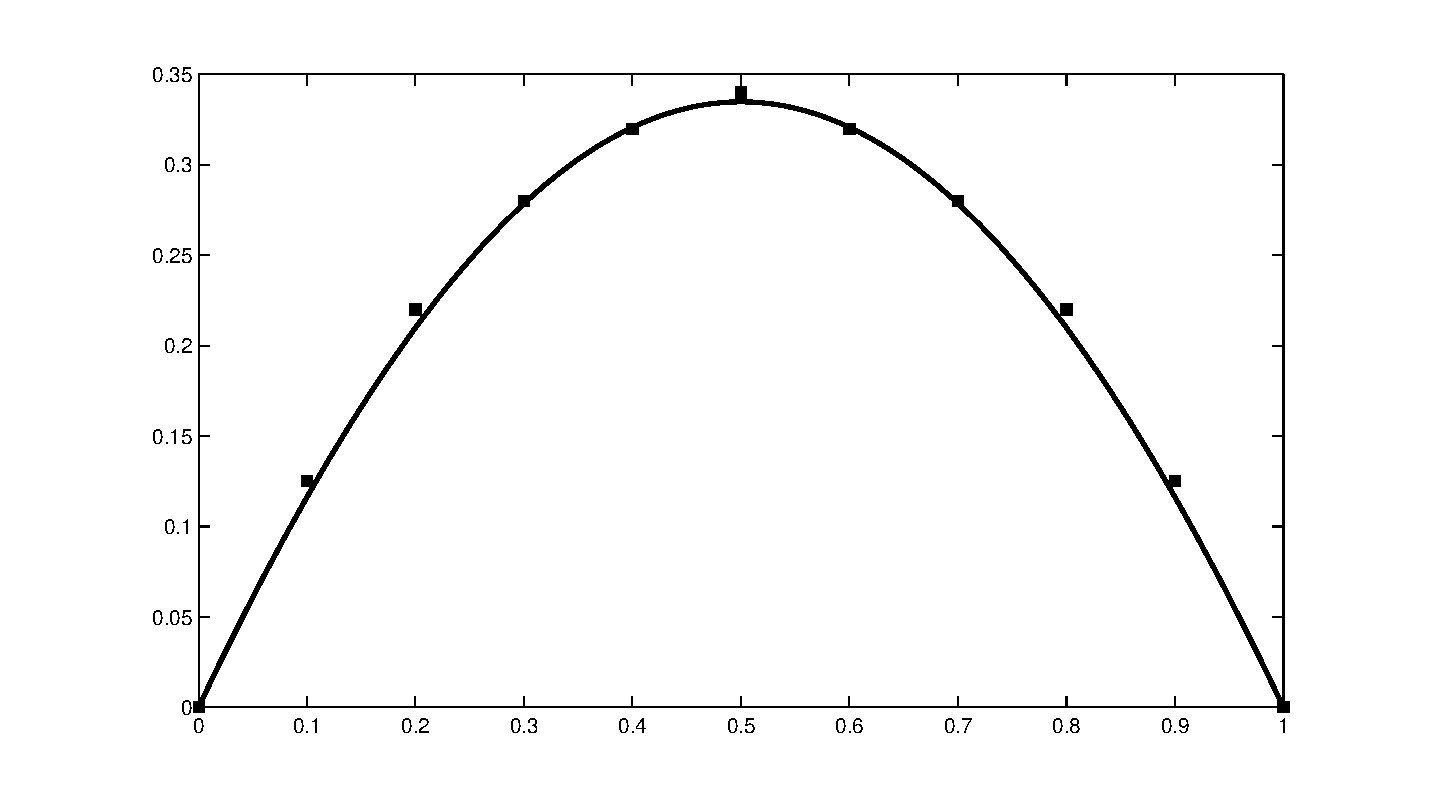
\includegraphics[scale=0.5]{./pic/6dcf.eps}
 \caption{扩散方程六点差分格式计算结果\label{fig:sm_ldcf}}
\end{figure}\par
\end{frame}
\begin{frame}{对流扩散方程}
考虑对流扩散方程
\begin{equation}\label{equ:cf_dkfangc}
	\dfrac{\partial u}{\partial t}+a\dfrac{\partial u}{\partial x}=\nu\dfrac{\partial^2 u}{\partial x^2}
\end{equation}
其中a、$\nu$ 为常数,$\nu>0$,给定初值
\begin{equation}
	u(x,0)=g(x)
\end{equation}
我们利用差分方法得到了一组差分方程,然后利用追赶法求解.
\end{frame}
\begin{frame}
\begin{figure}[h]
\centering
\includegraphics[scale=0.30]{./pic/dlfc.eps}
\end{figure}\par
\begin{figure}[h]
\centering
\includegraphics[scale=0.30]{./pic/dlfc2.eps}
\end{figure}
\end{frame}
\begin{frame}
考虑这样的多维方程
\begin{equation}\label{eq:sm_dw}
R_d\dfrac{\partial C}{\partial t}+v_i\dfrac{\partial C}{\partial x_i}=\dfrac{\partial}{\partial x_i}(D_{ij}\dfrac{\partial C}
{\partial x_j})-\mu C+\lambda,\quad (i,j=1,2)
\end{equation}
我们采用有限元法来求解这个方程,不考虑对流项.
\end{frame}
\begin{frame}{巨大芽孢杆菌}
\begin{figure}[h]
\subfloat[$t=10$]{\centering\includegraphics[scale=0.2]{./pic/01.png}}
\subfloat[$t=100$]{\centering\includegraphics[scale=0.2]{./pic/01-100.png}}
\subfloat[$t=600$]{\centering\includegraphics[scale=0.2]{./pic/01-600.png}}
%\caption{巨大芽孢杆菌的仿真结果}\label{pic:1}
\end{figure}
%\begin{figure}
%\setlength{\abovecaptionskip}{0pt}
%\setlength{\belowcaptionskip}{0pt}
%\subfloat[巨大芽孢杆菌]{\centering\includegraphics[scale=0.2]{./pic/01.png}}
%\subfloat[假单胞菌]{\centering\includegraphics[scale=0.2]{./pic/02.png}}
%\subfloat[大肠杆菌]{\centering\includegraphics[scale=0.2]{./pic/03.png}}
%
%\end{figure}
\end{frame}
\begin{frame}{假单胞菌}
\begin{figure}[h]
\subfloat[$t=10$]{\centering\includegraphics[scale=0.2]{./pic/02.png}}
\subfloat[$t=100$]{\centering\includegraphics[scale=0.2]{./pic/02-100.png}}
\subfloat[$t=600$]{\centering\includegraphics[scale=0.2]{./pic/02-600.png}}
%\caption{巨大芽孢杆菌的仿真结果}\label{pic:1}
\end{figure}
\end{frame}
\begin{frame}{大肠杆菌}
\begin{figure}[h]
\subfloat[$t=10$]{\centering\includegraphics[scale=0.2]{./pic/03.png}}
\subfloat[$t=100$]{\centering\includegraphics[scale=0.2]{./pic/03-100.png}}
\subfloat[$t=600$]{\centering\includegraphics[scale=0.2]{./pic/03-600.png}}
%\caption{巨大芽孢杆菌的仿真结果}\label{pic:1}
\end{figure}
\end{frame}
\begin{frame}{枯草芽孢杆菌}
\begin{figure}[h]
\subfloat[$t=10$]{\centering\includegraphics[scale=0.2]{./pic/04.png}}
\subfloat[$t=100$]{\centering\includegraphics[scale=0.2]{./pic/04-100.png}}
\subfloat[$t=600$]{\centering\includegraphics[scale=0.2]{./pic/04-600.png}}
%\caption{巨大芽孢杆菌的仿真结果}\label{pic:1}
\end{figure}
\end{frame}
\begin{frame}{金黄色葡萄球菌}
\begin{figure}[h]
\subfloat[$t=10$]{\centering\includegraphics[scale=0.2]{./pic/05.png}}
\subfloat[$t=100$]{\centering\includegraphics[scale=0.2]{./pic/05-100.png}}
\subfloat[$t=600$]{\centering\includegraphics[scale=0.2]{./pic/05-600.png}}
%\caption{巨大芽孢杆菌的仿真结果}\label{pic:1}
\end{figure}
\end{frame}
\begin{frame}{微球菌}
\begin{figure}[h]
\subfloat[$t=10$]{\centering\includegraphics[scale=0.2]{./pic/05.png}}
\subfloat[$t=100$]{\centering\includegraphics[scale=0.2]{./pic/05-100.png}}
\subfloat[$t=600$]{\centering\includegraphics[scale=0.2]{./pic/05-600.png}}
%\caption{巨大芽孢杆菌的仿真结果}\label{pic:1}
\end{figure}
\end{frame}
\section{结论与展望}
\begin{frame}{总结}
在本研究中,我们讨论了
\begin{fsitemize}
\item 扩散方程、对流方程、非齐次方程的精确解方法;
\item 中心差分格式、迎风差分格式等差分格式及相应的隐格式的形式、稳定性、误差;
\item 差分格式的求解方法;
\item 算子分裂法求解复杂偏微分方程的方法.
\end{fsitemize}
% 在本课题中我们以此讨论了扩散方程、对流方程、对流扩散方程和对流扩散反应方程的解析解和数值解的求解方法.
% 同时利用算子分裂法将三维空间模型分解为简单的微分方程,求得其数值解.这项工作给我们了解微生物在土壤中
% 的运移规律打下了基础.\par
\end{frame}
\begin{frame}{展望}
利用控制理论中关于分布参数系统的相关理论,找到合适的被控变量和操纵变量,根据数学模型推得合适的控制规律
和参数,从而对微生物的运移过程进行控制.
\end{frame}
	\section*{}
	\begin{frame}
	\begin{center}
	\Large
	谢谢!\par
	欢迎提问
	\end{center}
	\end{frame}
\end{document}